% THIS IS SIGPROC-SP.TEX - VERSION 3.1
% WORKS WITH V3.2SP OF ACM_PROC_ARTICLE-SP.CLS
% APRIL 2009
%
% Questions regarding SIGS should be sent to
% Adrienne Griscti ---> griscti@acm.org
%
% Questions/suggestions regarding the guidelines, .tex and .cls files, etc. to
% Gerald Murray ---> murray@hq.acm.org
%
% For tracking purposes - this is V3.1SP - APRIL 2009
%
% Copied from https://github.com/heathermiller/papers-documents/tree/master/rem2013

\documentclass{support/acm_proc_article-sp}
\usepackage{listings}
\usepackage{url}
\usepackage{support/bcprules}
\usepackage{support/prooftree}
\usepackage{support/math}
\usepackage{multicol}
\usepackage{caption}
\usepackage{subcaption}
\usepackage[normalem]{ulem}
\usepackage{color}
\usepackage{graphicx}
\usepackage{hyperref}

\renewcommand{\thesubsection}{\thesection.\alph{subsection}}

\definecolor{blue}{rgb}{0,0,0.5}
\definecolor{red}{rgb}{0.6,0,0}
\definecolor{green}{rgb}{0,0.5,0}
\definecolor{grey}{rgb}{0.2,0.2,0.2}

\lstdefinelanguage{Python}{
keywords={typeof, null, catch, switch, in, int, str, float, self},
keywordstyle=\color{blue}\bfseries,
ndkeywords={boolean, throw, import},
ndkeywords={return, class, if ,elif, endif, while, do, else, True, False , catch, def},
ndkeywordstyle=\color{blue}\bfseries,
identifierstyle=\color{red},
sensitive=false,
comment=[l]{\#},
morecomment=[s]{/*}{*/},
commentstyle=\color{green}\ttfamily,
stringstyle=\color{green}\ttfamily,
}

\lstset{language=Python}

% comments and notes
\newcommand{\comment}[1]{}
\newcommand{\note}[1]{{\bf $\clubsuit$ #1 $\spadesuit$}}
\newcommand{\ifreport}[1]{#1}
%\newcommand{\ifreport}[1]{}

\newcommand{\todo}{{\bf \colorbox{red}{\color{white}TODO:}}}
\newcommand{\ie}{{\em i.e.,~}}
\newcommand{\eg}{{\em e.g.,~}}
\newcommand{\term}[1]{\mbox{\texttt{#1}}}
\newcommand{\itl}[1]{\mbox{\textit{#1}}}

% commas and semicolons
\newcommand{\comma}{,\,}
\newcommand{\commadots}{\comma \ldots \comma}
\newcommand{\semi}{;\mbox{;};}
\newcommand{\semidots}{\semi \ldots \semi}

% spacing
\newcommand{\gap}{\quad\quad}
\newcommand{\biggap}{\quad\quad\quad}
\newcommand{\nextline}{\\ \\}
\newcommand{\htabwidth}{0.5cm}
\newcommand{\tabwidth}{1cm}
\newcommand{\htab}{\hspace{\htabwidth}}
\newcommand{\tab}{\hspace{\tabwidth}}
\newcommand{\linesep}{\ \hrulefill \ \smallskip}

\newcommand{\sectionline}{%
\nointerlineskip \vspace{\baselineskip}%
\hspace{\fill}\rule{0.5\linewidth}{.7pt}\hspace{\fill}%
\par\nointerlineskip \vspace{\baselineskip}
}

% figures
\newcommand{\figurebox}[1]
{\fbox{\begin{minipage}{\textwidth}
           #1 \medskip
\end{minipage}}}
\newcommand{\twofig}[3]
{\begin{figure*}[t]
     #3\ \hrulefill\
        \caption{\label{#1}#2}
\end{figure*}}
\newcommand{\boxfig}[3]
{\begin{figure*}
     \figurebox{#3\caption{\label{#1}#2}}
\end{figure*}}
\newcommand{\figref}[1]
{Figure~\ref{#1}}

% arrays
\newcommand{\ba}{\begin{array}}
\newcommand{\ea}{\end{array}}
\newcommand{\bda}{\[\ba}
\newcommand{\eda}{\ea\]}
\newcommand{\ei}{\end{array}}
\newcommand{\bcases}{\left\{\begin{array}{ll}}
\newcommand{\ecases}{\end{array}\right.}

\pagenumbering{arabic}
\begin{document}

    \title{Hot Topics in Machine Learning (HWS17) \\ Assignment 3: Graphical Models}

    \numberofauthors{1}
    \author{
    \alignauthor
    Steffen Schmitz\\
    \affaddr{University of Mannheim}\\
    \affaddr{stefschm@mail.uni-mannheim.de}
    }

    \maketitle

    %%%%%%%%%%%%%%%%%%%%%%%%%%%%%%%%%%%%%%%%%%%%%%%%%%%%
    %%
    %% 1) INFERENCE IN FACTOR GRAPHS
    %%
    %%%%%%%%%%%%%%%%%%%%%%%%%%%%%%%%%%%%%%%%%%%%%%%%%%%%

    \section{Inference in Factor Graphs}

    \textbf{Task.} The goal of this assignment is to implement and experiment with various inference methods for factor graphs.
    We use the misconception example throughout;
    refer to the lecture slides for details.

    %%%%%%%%%%%%%%%%%%%%%%%%%%%%%%%%%%%%%%%%%%%%%%%%%%%%
    %%
    %% 1.a) NAIVE INFERENCE
    %%
    %%%%%%%%%%%%%%%%%%%%%%%%%%%%%%%%%%%%%%%%%%%%%%%%%%%%

    \subsection{Naive}

    \textbf{Task.} Implement a function \emph{naive} that takes a factor graph and outputs the full joint distribution
    of its variables using naive inference.

    To compute the full joint distribution for a factor graph we have to create all possible combinations between variables, and,
    therefore, compute the product of all factors contained in the graph.
    \begin{equation*}
        \tilde{P}(X) = \prod_{i = 1}^{m} \phi_i(X_i)
    \end{equation*}
    Afterwards this must be normalized so that the values sum up to one and form a probability.

    %%%%%%%%%%%%%%%%%%%%%%%%%%%%%%%%%%%%%%%%%%%%%%%%%%%%
    %%
    %% 1.b) VARIABLE ELIMINATION
    %%
    %%%%%%%%%%%%%%%%%%%%%%%%%%%%%%%%%%%%%%%%%%%%%%%%%%%%

    \subsection{Variable Elimination}

    \textbf{Task.} Implement a function eliminate that takes a factor graph and uses variable elimination to eliminate
    a specified set of variables.
    Provide in your solution the factor graphs in which (i) \{ $A$ \}, (ii) \{ $A, B$ \},
    and (iii) \{ $A, B, C$ \} have been eliminated.

    We use variable elimination to remove non-query variables from the graph.
    This means that we remove variables we are not interested in, to reduce the complexity of our factor graph.
    We do this by marginalizing out the non-query variable from all factors that depend on it.
    See Figure \ref{fig:eliminate} for the Python implementation.
    \begin{figure}[!htbp]
        \centering
        \lstset{numbers=none,xleftmargin=0em}
        \lstinputlisting{listings/eliminate.py}
        \caption{Variable Elimination.}
        \label{fig:eliminate}
    \end{figure}

    Given the Factor Graph from the lecture we can now remove non-query variables \{ $A$ \}, \{ $A, B$ \} and \{ $A, B, C$ \},
    respectively.
    We do this by multiplying all factors $\phi$ that depend on the variable that we want to remove and fixing the value
    of the variable while computing the factor product.
    This way we derive a new factor that takes the place of all factors that depended on the non-query variable.
    This results in the Tables \ref{table:elim-a}, \ref{table:elim-ab} and \ref{table:elim-abc}.
    \begin{table}[!htbp]
        \begin{center}
            \begin{tabular}{ c c c | c }
                Bob & Charlie & Debbie & value \\
                \hline
                0 & 0 & 0 & 0.0416699 \\
                0 & 0 & 1 & 0.180509 \\
                0 & 1 & 0 & 0.0416699 \\
                0 & 1 & 1 & 1.80509e-05 \\
                1 & 0 & 0 & 7.08152e-05 \\
                1 & 0 & 1 & 0.0139548 \\
                1 & 1 & 0 & 0.708152 \\
                1 & 1 & 1 & 0.0139548 \\
            \end{tabular}
        \end{center}
        \caption{Elimination of (i) \{ $A$ \}.}
        \label{table:elim-a}
    \end{table}

    \begin{table}[!htbp]
        \begin{center}
            \begin{tabular}{ c c | c }
                Charlie & Debbie & value \\
                \hline
                0 & 0 & 0.0417407 \\
                0 & 1 & 0.194464 \\
                1 & 0 & 0.749822 \\
                1 & 1 & 0.0139728 \\
            \end{tabular}
        \end{center}
        \caption{Elimination of (ii) \{ $A, B$ \}.}
        \label{table:elim-ab}
    \end{table}

    \begin{table}[!htbp]
        \begin{center}
            \begin{tabular}{ c | c }
                Debbie & value \\
                \hline
                0 & 0.791563 \\
                1 & 0.208437 \\
            \end{tabular}
        \end{center}
        \caption{Elimination of (iii) \{ $A, B, C$ \}.}
        \label{table:elim-abc}
    \end{table}

    %%%%%%%%%%%%%%%%%%%%%%%%%%%%%%%%%%%%%%%%%%%%%%%%%%%%
    %%
    %% 1.c) GIBBS SAMPLING
    %%
    %%%%%%%%%%%%%%%%%%%%%%%%%%%%%%%%%%%%%%%%%%%%%%%%%%%%

    \subsection{Gibbs Sampling}
    \label{sec:gibbs-sampling}

    \textbf{Task.} Implement a function gibbs that takes a factor graph and uses Gibbs sampling to resample the values
    of a specified set of variables.
    In particular, to resample variable $X$, compute $P(X | \mbox{ values of all other variables})$ and sample from this conditional
    distribution. \\
    Suppose $A=1$, $B=0$, $C=1$, $D=0$.
    Provide in your solution the conditional distributions for (i) $A$, (ii) $B$, (iii) $C$, and (iv) $D$ conditioned on the
    just specified values of the other variables.
    If you have trouble implementing function gibbs, proceed manually and describe each step.
    Otherwise, it suffices to specify the resulting distributions.

    We sample the value of exactly one variable at a time while keeping the values of the other variables fixed.
    This is done by creating the conditional probability table of the variable that we want to sample from and looking
    up the probability, depending on the other, known values. \cite[p.838]{Murphy:2012:MLP:2380985}

    The approach of using the conditional probability table is often faster than using the full joint distribution,
    because it is possible to ignore all factors that contain only variables that are conditionally independent of the
    sampled variable. \cite[p.494f.]{Russell:2003:AIM:773294}

    See Figure \ref{fig:gibbs} for the Python implementation.
    \begin{figure}[!htbp]
        \centering
        \lstset{numbers=none,xleftmargin=0em}
        \lstinputlisting{listings/gibbs.py}
        \caption{Gibbs Sampling.}
        \label{fig:gibbs}
    \end{figure}

    If we apply this function to the given distribution with the fixed values stated in the task we get the sampled
    distributions in Tables \ref{table:gibbs-a}, \ref{table:gibbs-b}, \ref{table:gibbs-c} and \ref{table:gibbs-d}.

    \begin{table}[!htbp]
        \begin{center}
            \begin{tabular}{ c c c c }
                Anna & expected & observed & estimated \\
                \hline
                0 & 0.999667 & 999 & 0.999 \\
                1 & 0.000333222 & 1 & 0.001 \\
            \end{tabular}
        \end{center}
        \caption{Sample $A$ conditioned on $B$, $C$, $D$ (i).}
        \label{table:gibbs-a}
    \end{table}

    \begin{table}[!htbp]
        \begin{center}
            \begin{tabular}{ c c c c }
                Bob & expected & observed & estimated \\
                \hline
                0 & 0.000999001 & 0 & 0 \\
                1 & 0.999001 & 1000 & 1 \\
            \end{tabular}
        \end{center}
        \caption{Sample $B$ conditioned on $A$, $C$, $D$ (ii).}
        \label{table:gibbs-b}
    \end{table}

    \begin{table}[!htbp]
        \begin{center}
            \begin{tabular}{ c c c c }
                Charlie & expected & observed & estimated \\
                \hline
                0 & 0.5 & 523 & 0.523 \\
                1 & 0.5 & 477 & 0.477 \\
            \end{tabular}
        \end{center}
        \caption{Sample $C$ conditioned on $A$, $B$, $D$ (iii).}
        \label{table:gibbs-c}
    \end{table}

    \begin{table}[!htbp]
        \begin{center}
            \begin{tabular}{ c c c c }
                Debbie & expected & observed & estimated \\
                \hline
                0 & 0.5 & 505 & 0.505 \\
                1 & 0.5 & 495 & 0.495 \\
            \end{tabular}
        \end{center}
        \caption{Sample $D$ conditioned on $A$, $B$, $C$ (iv).}
        \label{table:gibbs-d}
    \end{table}

    %%%%%%%%%%%%%%%%%%%%%%%%%%%%%%%%%%%%%%%%%%%%%%%%%%%%
    %%
    %% 1.d) EXPERIMENTING WITH GIBBS SAMPLING
    %%
    %%%%%%%%%%%%%%%%%%%%%%%%%%%%%%%%%%%%%%%%%%%%%%%%%%%%

    \subsection{Experimenting with Gibbs Sampling}
    \label{sec:gibbs-experiments}

    \textbf{Task.} Investigate the quality of the estimated marginal distributions for various choices of $n$
    (keep $s = w = 0$ for now).
    To do so, compare the estimates with the exact result as well as with the estimates provided from n independent
    samples.
    Discuss your findings. \\
    Now fix $n = 1000$ and investigate the impact of values of $s$ and $w$.
    Discuss your findings.

    First we will look at the quality of estimates depending on the number of samples that we take.
    The independent sampling method takes a number of samples and a normalized distribution as its parameters
    and uses a multinomial distribution for random sampling that is parameterized with the probabilities from the input
    distribution.
    It runs $n$ randomized and independent experiments.

    Our Gibbs Sampling function samples one variable at a time and threats the other variables as a fixed value.
    In one of the $n$ runs it samples each variable exactly once.
    We reuse the method from Section \ref{sec:gibbs-sampling} here.

    Afterwards we compute the L1-Error to compare the exact result with our Gibbs- and the independent Sample.
    The L1-Error uses sum of absolute difference between two probabilities.

    The errors are shown graphically in Figure \ref{fig:gibbs-n}.
    The dotted lines show the errors for gibbs-sampling and the solid lines for the independent sampling.
    \begin{figure}[!htbp]
        \centering
        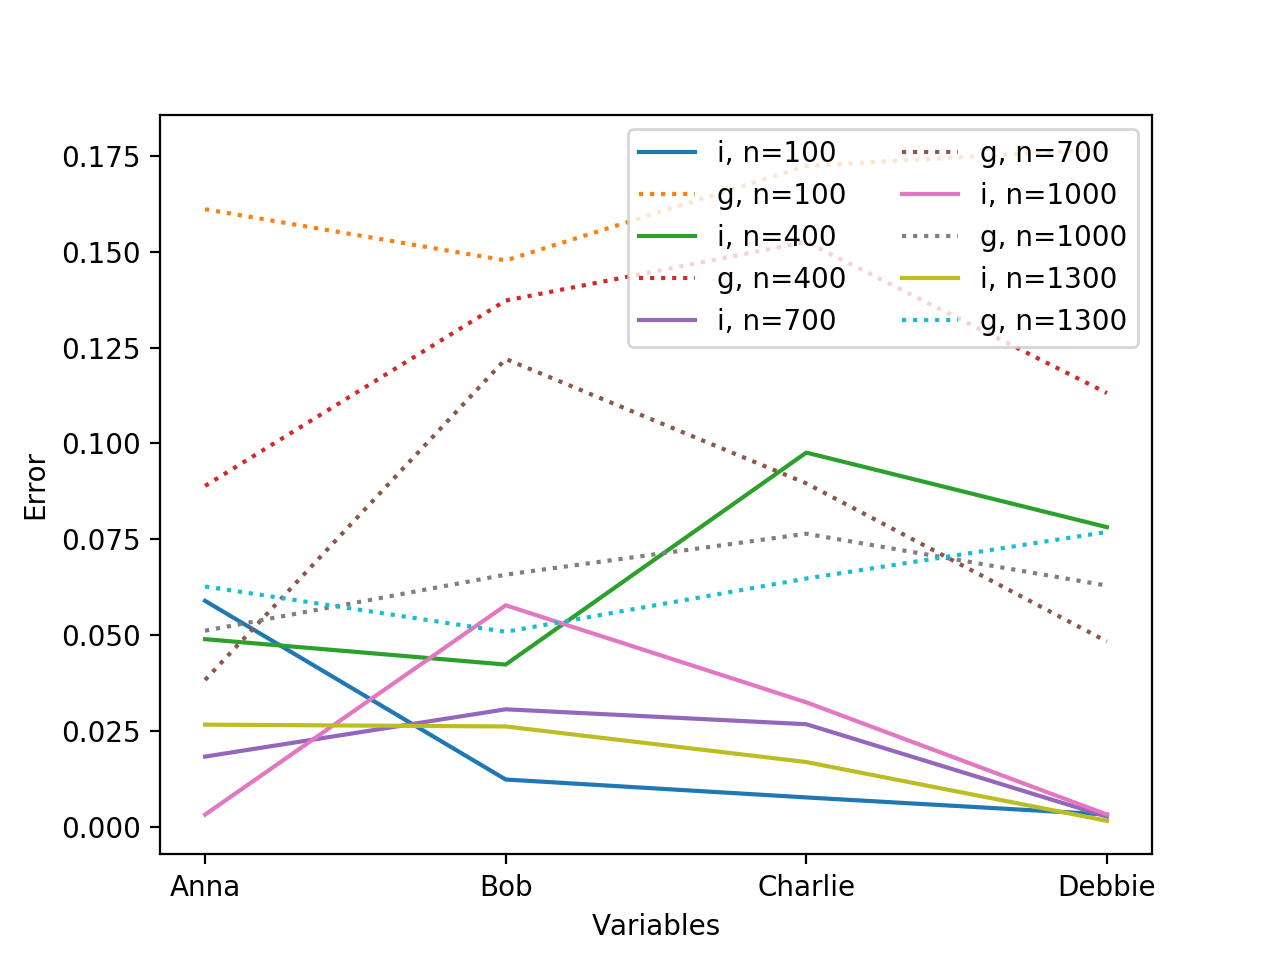
\includegraphics[width=8cm]{images/gibbs-n.png}
        \caption{Gibbs and independent sampling for $n$ samples.}
        \label{fig:gibbs-n}
    \end{figure}

    We can see that the error for the Gibbs-sampled distributions is usually higher than the one for the independently
    sampled distributions and decreases for both ways with the number of samples that we take.

    This can be explained by the missing burn-in phase of our Gibbs sampling model.
    Usually, it is necessary to skip the first examples to make the distribution "forget" its initial state \cite[p.856f.]{Murphy:2012:MLP:2380985}.
    It is also more likely to get a skewed distribution if you take a little number of samples due to the randomness.
    If many samples are collected the initial randomness averages out and approximates the true distribution \cite[p.96f.]{HoffPeterD2009Afci}.

    We conclude that an increasing number of samples decreases the error and the sampled distribution approximates the
    exact distribution for larger $n$.

    Now we will look at the influence of the warm-up (burn-in) phase and the skip.
    A warm-up of $m$ steps means that the first $m$ samples are simply dismissed and the collection of samples starts
    afterwards.
    The skip parameter specifies the number of runs that are ignored between runs that are used for sampling.
    A higher skip parameter means that the samples that are taken are more independent than on subsequent Gibbs-sample-runs
    and reduce the autocorrelation that is usually observed in Gibbs-sampling.

    The errors are shown in Figure \ref{fig:gibbs-ws} where dotted lines again represent the Gibbs-sampled errors.
    \begin{figure}[!htbp]
        \centering
        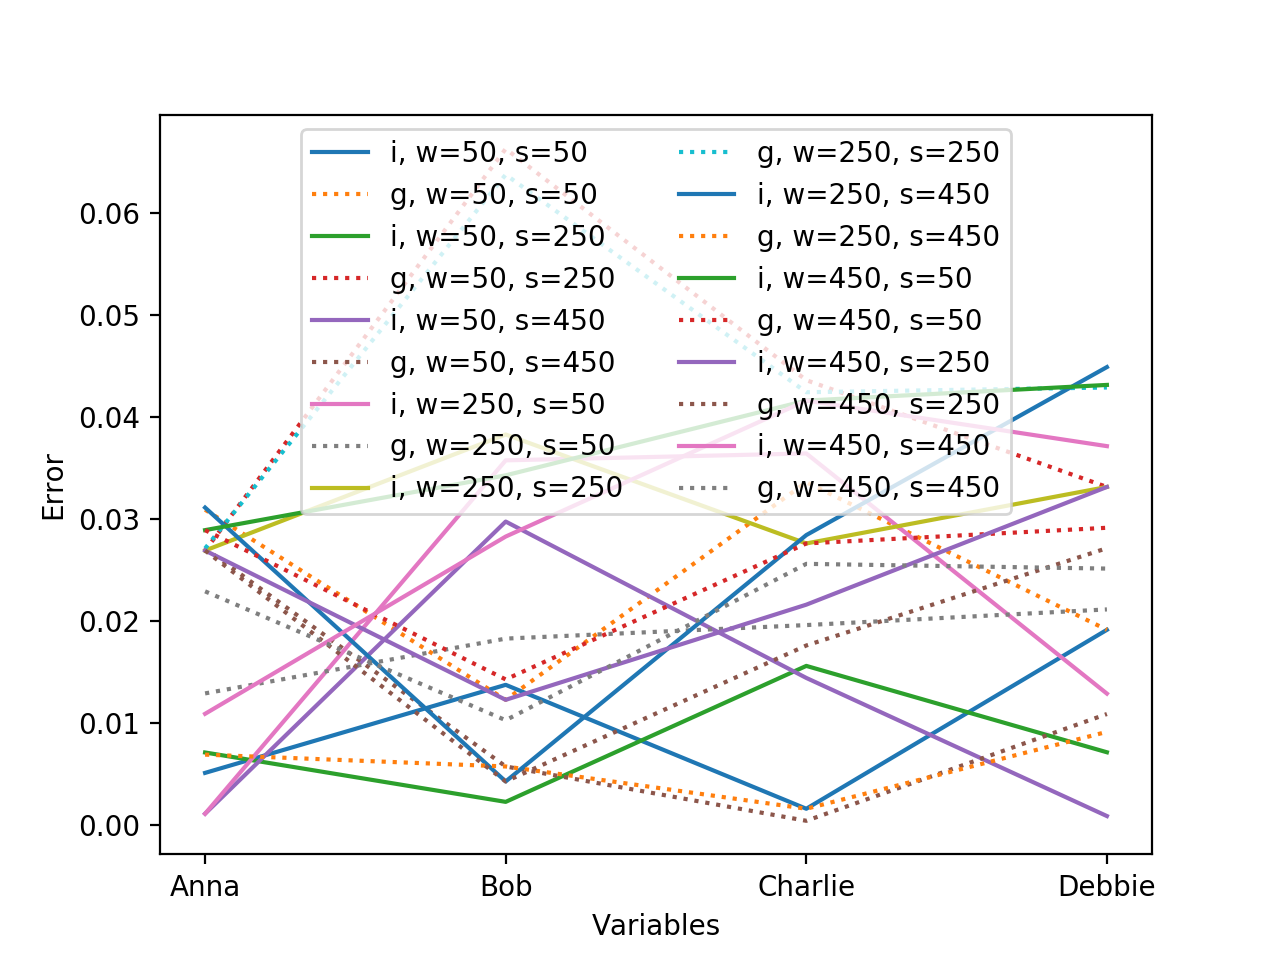
\includegraphics[width=8cm]{images/gibbs-ws.png}
        \caption{Gibbs and independent sampling for different warm-up and skip.}
        \label{fig:gibbs-ws}
    \end{figure}

    After the addition of a warm-up phase and skips we can not distinguish between the independently and Gibbs-sampled
    distributions anymore.
    This supports our initial intuition about the effects of a warm-up phase and the skip phase.
    The larger both parameters are, the more should our Gibbs-sample resemble the independent sample.

    %%%%%%%%%%%%%%%%%%%%%%%%%%%%%%%%%%%%%%%%%%%%%%%%%%%%
    %%
    %% 2) FACTOR GRAPHS AND NAIVE BAYES
    %%
    %%%%%%%%%%%%%%%%%%%%%%%%%%%%%%%%%%%%%%%%%%%%%%%%%%%%

    \section{Factor Graphs and Naive Bayes}

    The markov network graph and factor graph for a general Naive Bayes model can be represented as in Figure \ref{fig:nba}.
    We can see that all features $X$ are conditionally independent to each other given $Y$.
    \begin{figure}[!htbp]
        \centering
        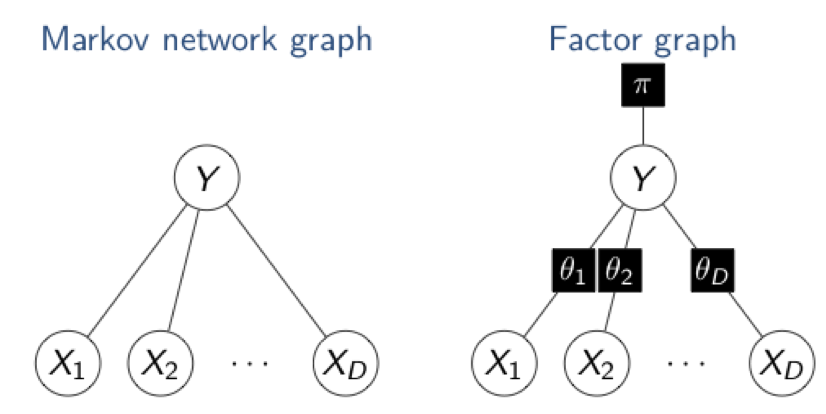
\includegraphics[width=8cm]{images/nba.png}
        \caption{General Naive Bayes Representation.}
        \label{fig:nba}
    \end{figure}

    %%%%%%%%%%%%%%%%%%%%%%%%%%%%%%%%%%%%%%%%%%%%%%%%%%%%
    %%
    %% 2.a) SAMPLE LABEL ONCE
    %%
    %%%%%%%%%%%%%%%%%%%%%%%%%%%%%%%%%%%%%%%%%%%%%%%%%%%%

    \subsection{Sample label once}

    \textbf{Task.} Suppose we use Gibbs sampling to sample $P(Y | X)$ once.
    Describe informally the result.

    As already displayed on the right hand side of Figure \ref{fig:nba} the variable $Y$ depends on all variables $X$ and,
    therefore, has a common factor with each of those variables.
    To sample from $Y$ we need to compute the product of all factors that include $Y$, which is, in the Naive Bayes network,
    every included factor.
    \begin{equation*}
        \prod_{i = 1}^D \phi_i (Y, X_i) = P(Y, X_1, X_2,\mbox{ ... }, X_D)
    \end{equation*}
    This is equal to the full joint distribution of the network \cite[p.104f.]{Koller:2009:PGM:1795555}, which can be
    extremely large and infeasible to compute efficiently \cite[p.477]{Russell:2003:AIM:773294}.

    Assuming that we are able to compute the full joint distribution we would get a random sample in the range $[0, 9]$
    with the probabilities that we looked up in the full joint distribution table based on the values of all variables
    in $\mathbf{X}$.

    %%%%%%%%%%%%%%%%%%%%%%%%%%%%%%%%%%%%%%%%%%%%%%%%%%%%
    %%
    %% 2.b) SAMPLE LABEL N-TIMES
    %%
    %%%%%%%%%%%%%%%%%%%%%%%%%%%%%%%%%%%%%%%%%%%%%%%%%%%%

    \subsection{Sample label n-times}

    \textbf{Task.} Suppose we compute $n$ Gibbs samples $y_1, ..., y_n$ by sampling $P(Y | X)$ $n$ times using Gibbs sampling.
    Are these $n$ samples dependent or independent (conditioned on $X$)?
    Discuss briefly.

    If we sample the $P(Y | X)$ multiple times the resulting values $y_1,..., y_n$ are independent of each other
    conditioned on $X$, because they are not used to compute the probability for a randomized sample $y_i$.
    The autocorrelation between samples in Gibbs sampling stems from the fact that all values are kept constant except one.
    If only one value is sampled it is still randomized based on the other, fixed parameters.

    %%%%%%%%%%%%%%%%%%%%%%%%%%%%%%%%%%%%%%%%%%%%%%%%%%%%
    %%
    %% 2.c) SAMPLE INPUT
    %%
    %%%%%%%%%%%%%%%%%%%%%%%%%%%%%%%%%%%%%%%%%%%%%%%%%%%%

    \subsection{Sample input}
    \label{sec:sample-input}

    \textbf{Task.} Suppose we compute a Gibbs sample of $P(X | Y)$.
    Describe informally the result.

    If we sample some input values $x_1,...,x_D$ exactly once per value we will get a random pixel color per value with
    the probability that the trained Naive Bayes model assigned this pixel for the specific value for $Y$.
    Our graph model encodes the Naive Bayes assumption, which means that every sampled value $x_i$ is independent of all
    other values and, therefore, it does not make a difference if they are initialized to zero or already sampled.

    %%%%%%%%%%%%%%%%%%%%%%%%%%%%%%%%%%%%%%%%%%%%%%%%%%%%
    %%
    %% 2.d) SAMPLE INPUT N-TIMES
    %%
    %%%%%%%%%%%%%%%%%%%%%%%%%%%%%%%%%%%%%%%%%%%%%%%%%%%%

    \subsection{Sample input n-times}

    \textbf{Task.} Suppose we compute $n$ Gibbs samples $x_1,...,x_D$ by sampling $P(X | Y)$ $n$ times using Gibbs sampling.
    Are these $n$ samples dependent or independent (conditioned on $Y$)?
    Discuss briefly.

    As we already said in Section \ref{sec:sample-input} all input variables $x_1,...,x_D$ are conditionally independent
    given $Y$.
    This means that the probability that we see a specific value for a sample $x_i$ is only depending on the label $y$ and
    not on the other variables.
    It makes no difference if we sample once or multiple times.
    The generated feature vectors will not be correlated.

    %%%%%%%%%%%%%%%%%%%%%%%%%%%%%%%%%%%%%%%%%%%%%%%%%%%%
    %%
    %% 2.e) SAMPLE INPUT AND LABEL
    %%
    %%%%%%%%%%%%%%%%%%%%%%%%%%%%%%%%%%%%%%%%%%%%%%%%%%%%

    \subsection{Sample input and label}

    \textbf{Task.} Suppose we compute $n$ Gibbs samples $(y_1,\mathbf{x}_1),...,(y_n,\mathbf{x}_n)$ by sampling $P(X,Y)$ $n$ times using Gibbs sampling.
    These $n$ samples will be dependent.
    Do you expect to see each class in roughly $\frac{n}{10}$ samples?
    Why or why not?

    Let's assume that we first sample an input feature vector from a given label and then sample turn wise.
    The first input vector will resemble the input label and the next sampled label will likely be closely related
    to the generated feature vector.
    We, therefore, have a correlation between the generated samples.

    As we have discussed in Section \ref{sec:gibbs-experiments} it is possible to reduce this correlation by introducing a skip
    and using a warm-up phase to "forget" our initial input.
    This may suffice to approach the true distribution of roughly $\frac{n}{10}$ samples per category.

    Some number are very different from others, e.g. 1 and 7 compared to 0.
    I would expect we see numbers that are similar to our initial input more often than ones that are highly different,
    although this effect may reduce for a very large number of samples.

    %%%%%%%%%%%%%%%%%%%%%%%%%%%%%%%%%%%%%%%%%%%%%%%%%%%%
    %%
    %% 2.f) NAIVE INFERENCE
    %%
    %%%%%%%%%%%%%%%%%%%%%%%%%%%%%%%%%%%%%%%%%%%%%%%%%%%%

    \subsection{Naive inference}

    \textbf{Task.} Can we run (in feasible time) naive inference on this factor graph?
    Can we eliminate all variables in $X$?
    Or just variable $Y$?
    In each case, why or why not?

    We can not run naive inference on the graph for the same reason that it is not possible to sample $Y$.
    We need to compute the full joint distribution which would have a complexity of $O(2^n)$ for binary variables -
    and our variables are not binary.

    It is not feasible to eliminate all variables in $X$ as we would need to create the corresponding factors
    and marginalize the variable out which also has an exponential complexity and blows up quickly.

    The same holds true for $Y$ as all values in $X$ depend on it and have to be taken into account.

    %%%%%%%%%%%%%%%%%%%%%%%%%%%%%%%%%%%%%%%%%%%%%%%%%%%%
    %%
    %% 3) CONDITIONAL RANDOM FIELDS
    %%
    %%%%%%%%%%%%%%%%%%%%%%%%%%%%%%%%%%%%%%%%%%%%%%%%%%%%

    \section{Conditional Random Fields}

    \textbf{Task.} The goal of this assignment is to apply linear-chain conditional random fields (CRF) to a simplified
    variant of the named entity recognition task.
    We use the Reuters-128 dataset for this task.
    The dataset contains multiple documents, in which each word is annotated with a label indicating whether the word
    is part of a named entity (label=1) or not (label=0).

    %%%%%%%%%%%%%%%%%%%%%%%%%%%%%%%%%%%%%%%%%%%%%%%%%%%%
    %%
    %% 3.a) ADDITIONAL FEATURES
    %%
    %%%%%%%%%%%%%%%%%%%%%%%%%%%%%%%%%%%%%%%%%%%%%%%%%%%%

    \subsection{Additional Features}

    \textbf{Task.} Provide additional features to the CRF that help to improve prediction performance.
    Which prediction performance can you achieve?

    The initial feature set that is already included in the code samples achieved 0.96 for precision, recall and the
    F1-Score.
    It included features like the Part of Speech (POS) Tag for the current, the previous and the next word and the
    position in the sentence (beginning or end).
    In this section we will try out more features to improve the prediction accuracy of our model.

    One feature that comes naturally to the mind when talking about named entities is the capitalization.
    Usually the only thinks that are capitalized in english sentences, excluding the first word, are special entities.
    As we already have a feature that tracks if the word is the first in a sentence we only focus on capitalization and
    add it.

    An additional feature might be that named entities often consist of multiple words, e.g. "Deputy U.S. Trade Representative
    Michael Smith", which may indicate that a capitalized word followed by another one means that both are part of a named
    entity.
    We introduce the feature "neighborAndSelfCapitalized" that checks if the current word and the word in front or behind
    are capitalized.
    We do not use a bigger scope, because Tkachenko and Simanovsky found that for most features a sliding window of three
    words provides the best result \cite{DBLP:conf:konvens:TkachenkoS12} and it would increase complexity.

    We also check if the word contains any digits [0, 1, ..., 9], numbers [one, two, ..., nine] or any other non-alphabetical
    characters, e.g. \$, \%, ;, @ etc.
    This may include non-standard words that are sometimes used for corporation names or product names, e.g. "OneDrive",
    "cloud9" or "@Home Network".

    The last included feature is about suffixes that usually indicate a noun, like -ness, -ship or -ion.
    Here we use the cambridge dictionary\footnote{\href{https://dictionary.cambridge.org/grammar/british-grammar/word-formation/suffixes}{https://dictionary.cambridge.org/suffixes}}
    for a list of possible suffixes.

    Applying this features we get an improvement 0.02 for the precision in predicting true labels and an improvement
    of 0.01 for the overall F1-Score.
    As the initial estimate was already pretty good, this is a solid improvement.

    %%%%%%%%%%%%%%%%%%%%%%%%%%%%%%%%%%%%%%%%%%%%%%%%%%%%
    %%
    %% 3.b) FEATURE INSPECTION
    %%
    %%%%%%%%%%%%%%%%%%%%%%%%%%%%%%%%%%%%%%%%%%%%%%%%%%%%

    \subsection{Feature Inspection}

    \textbf{Task.} Investigate the importance of each feature for prediction by inspecting its weight.
    Which features are important?
    Is it intuitive to you why these features are important?
    Which of your newly added features from a) helped most?

    The most important features are related to punctuation marks.
    If a feature has a trailing comma or a leading opened bracket it is more likely to be a named entity (weight 6.70205
    and 4.19538, respectively).
    A closed bracket in front an indicator for a non-named entity (weight 2.13726).
    It seems very intuitive that a word before a comma is a named entity, as it is likely that the following relative clause
    describes the entity in more detail.
    After the closed bracket it is also intuitive that a non-named entity follows, because the sentence is usually
    continued after the insertion.

    Although we initially estimated that a digit in the name is a sign of a named entity the weights show that it is more
    likely to be something else (weight 3.38014).
    The weight is similar to the preposition and verb features that are also strong indicators for a label of 0.

    The strongest self-created feature that indicates a label of 1 is as expected the capitalization with a weight of 2.45379.

    All in all most of the features behave as expected and lead to a solid F1-Score with a slight improvement related to
    the newly added ones.

    %%%%%%%%%%%%%%%%%%%%%%%%%%%%%%%%%%%%%%%%%%%%%%%%%%%%
    %%
    %% BIBLIOGRAPHY
    %%
    %%%%%%%%%%%%%%%%%%%%%%%%%%%%%%%%%%%%%%%%%%%%%%%%%%%%

    \bibliographystyle{abbrv}
    \bibliography{support/bib}

\end{document}
